\section{Biases}
\label{sec:biases}

In this section, we will present an updated central bias distribution (using a truncated Gaussian); explore the degree of asymmetry in viewing positions, and describe the saccadic flow model. 



%%%%%%%%%%%%%%%%%%%%%%%%%%%%%%%%%%%%%%%%%%%%%%%%%%%%%%%%%%
\subsection{Modelling Methods}
%%%%%%%%%%%%%%%%%%%%%%%%%%%%%%%%%%%%%%%%%%%%%%%%%%%%%%%%%%

In this section, we will give an overview of the methods and data used for the saccadic flow modelling.

\subsubsection{Datasets}

We will uses a number of previously published datasets. The models will be trained on a subset of the 10 datasets used in \cite{clarke-tatler2014}. These data are taken from \cite{clarke2013, tatler2005, tatler2007, yun2013, einhauser2008,judd2009}. The inital saccade after image onset ($9.1\%$ of the data) are excluded, giving us a total of 159,226 saccades. We chose to remove the data from \cite{asher2013} from our training set as the images have an aspect ratio of 5:4, whereas the rest of the data in our training set has an aspect ratio of 4:3. The pedestrian search dataset \citep{ehinger2009} was removed from the training set as previous analysis \citep{clarke-tatler2014} shows that it appears to be biased compared to the other datasets. Both these datasets are now used as test sets to evaluate how well our models generalise. 

We also add a number of other datasets to our test suite collection. 
\begin{itemize}
\item \cite{clarke2009} has a dataset of fixations made during a visual search for a target on a homogeneous textured background (i.e. target in noise). This dataset differs from the previous in that there is no semantic image content in the scene, and the stimuli had a 1:1 aspect ratio. \\

\item \cite{greene-wolfe2012} released a dataset of observers viewing square greyscale photographs.

\item \cite{borji2015} recently released a very large ($\approx 0.625$million fixations, 2000 images) dataset collected over twenty different stimuli types. Given the size of this dataset, and the widescreen 16:9 aspect ratio, the evaluations on this dataset are presented seperately, and split by stimuli class.\\

\end{itemize}

An overview of the datasets used is given in Appendix Tables \ref{tab:datasets} and \ref{tab:setuptable}.

\subsubsection{Pre-processing}

As with \cite{clarke-tatler2014} we have normalised all fixations to the image frame, keeping the aspect ratio constant. ie, $(x,y)\in (-1.-1)\times(-a,a)$ with typically $a=0.75$. The initial fixations and saccades were not included in the analysis. Saccades with a start or end point falling outside of the image frame were also removed. 

When fitting saccadic flow models,  we \textit{mirrored} the set of fixations, but adding in reflected copies of the data (reflected in the horizontal, vertical and both midlines). This has two advantages. (i) It is an easy way to make saccadic flow biases in the horizontal or vertical directions. This is similar to how the central bias was defined \cite{clarke-tatler2014}, but by a different mechanism (with the central bias, the model fitting procedure is much simpler and so we just enforced zero mean and 0s in the covariance matrix). (ii) It increases the amount of data available for fitting by a factor of four. This is important as (due to the central bias) there are relatively few saccades that originate from the corners of the images. By equating all corners, we can pool the data and obtain more stable estimates for the underlying distribution. 


The downside of mirroring saccades in this manner is that our model of saccadic flow will be insensitive to the \textit{leftwards} bias in natural scene viewing \citep{nuthmann-matthias2014}. This will be discussed in Section \ref{sec:LeftRight}. Similary, as ignore the timecourse of saccades we will not capture \textit{corase-to-fine} dynamics (discussed previous in Section \ref{sec:humanComp}).

We will model and discuss saccadic flow, coarse-to-fine, and left v right. 

\subsection{Truncated Central Bias}

First, we will update the central bias from \cite{clarke-tatler2014} and use a truncated normal distribution. This is very straight forward. Re-fitting a multivariante gaussian to the data reduces the deviance in the central bias model by $0.06\%$. Usng a truncated Gaussian gives us an improvement of $7.28\%$. We can round the truncated Gaussian model to $\mu = (0,0)$, $\sigma=(0.3, 0; 0, 0.12)$ with no loss of precision. 

\subsection{Left v Right}
\label{sec:LeftRight}

Initially more fixations to the left half of the image \citep{nuthmann-matthias2014}. We replicate this here (Figure \ref{fig:leftrightDist}).

\begin{figure}
\centering
\subfigure{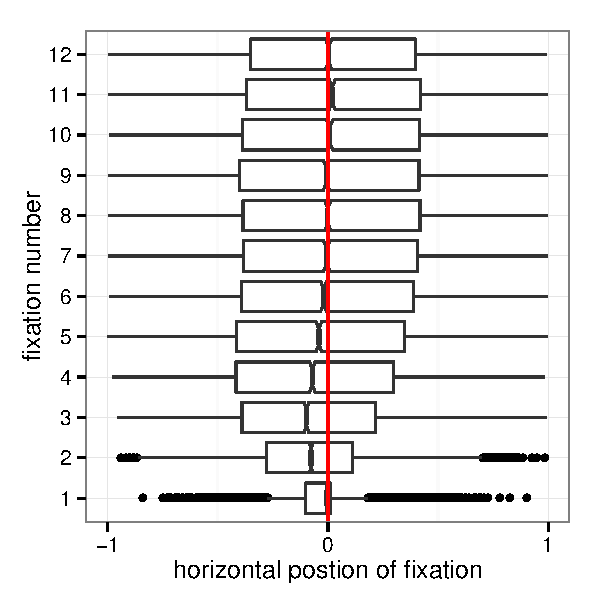
\includegraphics[width=3.6cm]{../scripts/leftVright/graphs/leftrightbias.pdf}}
\subfigure{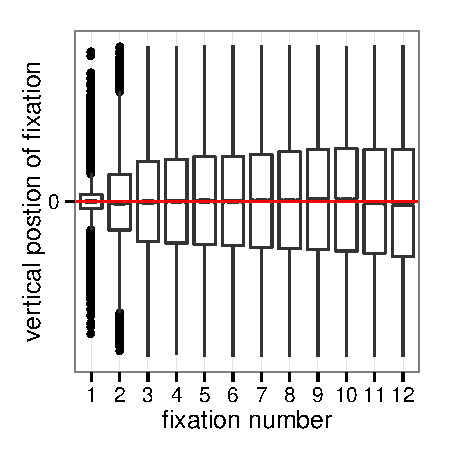
\includegraphics[width=3.6cm]{../scripts/leftVright/graphs/updownbias.pdf}}
\caption{Distribution of horizontal and vertical fixations by fixation number.}
\label{fig:leftrightDist}
\end{figure}

However, it has only a very small effect on explaining the varition over whole datasets: Figure \ref{fig:leftrightModelling}.

\begin{figure}
\centering
\subfigure[]{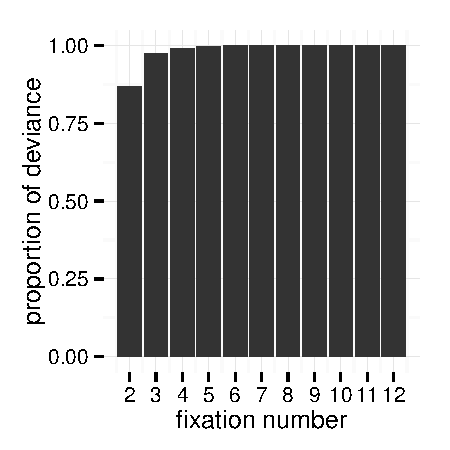
\includegraphics[width=4.1cm]{../scripts/leftVright/graphs/devRatio.pdf}}
\subfigure[]{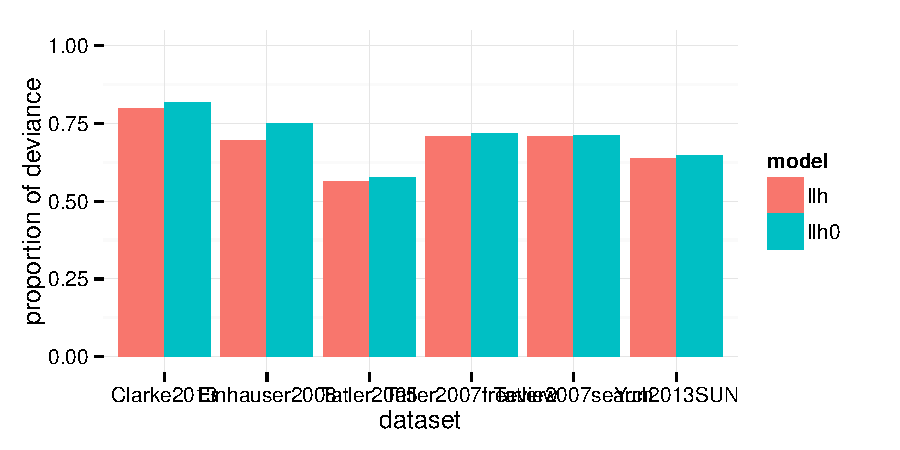
\includegraphics[width=8.2cm]{../scripts/leftVright/graphs/datasetComp.pdf}}
\caption{Modelling results}
\label{fig:leftrightModelling}
\end{figure}


Hence we will ignore this effect from now on. By treating everything as symmetrical, we lose very little explanitory power, while restricitng the number of parameters, or increasing the amount of data available (by mirroring fixations).

\subsection{Saccadic Flow}
\label{ModellingFlow}

Saccadic flow can be thought of as a generalisation of the central bias. Instead of computing the distribution of all saccadic endpoints in a dataset, we look at the distribution of saccade endpoints given the start points. So for a saccade from $(x_0, y_0)$ to $(x_1, y1)$ we want to model $p(x_1,y_1|x_0, y0)$ This is illustrated in Figure \ref{fig:empiricalSaccadicFlow}.

\subsubsection{Modelling}

To characterise how the distribution of saccadic endpoints varies with the start point, we used a sliding window approach. All saccades that originated in a $n\times n$ window were taken and used to fit a multivariate Gaussian distribution. This window was then moved over the stimuli in steps of $s=0.01$. Parameter sets estimated from windows containing less than 250 datapoints were removed. Multivariate polynomial regression was then used to fit 4-th order polynomials to each of the parameters. Robust estimation was used (\texttt{rlm} from the texttt{MASS} library) to stop the model fits being overly infleunced by outlier points from the image boundary. We experimented with varying the window size ($n\in\{0.05,0.1, 0.2\}$). However, as this parameter was found to have a negligible result, we only report the results for $n=0.05$.


\subsubsection{Results}

Figure \ref{fig:nParamsOverSpace} shows how the parameters for the multivariate Gaussian distribution vary over horizontal position for a selection of vertical positions. The regression coefficients given in Table \ref{tab:nParamModel} allow us to estimate the conditional probability of a saccade to $(x_1, y1)$ given the starting fixation $(x_0, y_0)$.

\begin{table*}
\centering
\begin{tabular}{c c}
parameter & equation \\
\hline
$\Omega_{x,x}$	& $= 0.33+ 0.38x^2 -0.29y^2 + 0.02x^4 + 0.22y^4$ \\ 
$\Omega_{x,y}$	& $=x + y + x^2 + y^2 + x^3 + y^3 + x^4 + y^4$ \\ 
$\Omega_{y,x}$	& $=x + y + x^2 + y^2 + x^3 + y^3 + x^4 + y^4$ \\ 
$\Omega_{y,y}$	& $=x + y + x^2 + y^2 + x^3 + y^3 + x^4 + y^4$ \\ 
\hline
$\alpha_{x^2}$		& $=x + y + x^2 + y^2 + x^3 + y^3 + x^4 + y^4$ \\ 
$\alpha_{y^2}$		& $=x + y + x^2 + y^2 + x^3 + y^3 + x^4 + y^4$ \\ 
\hline
$\nu$			& $=x + y + x^2 + y^2 + x^3 + y^3 + x^4 + y^4$ \\ 
\end{tabular}
\caption{Parameter model - clearly I still have to fill in all the coefficients!}
\label{tab:nParamModel}
\end{table*}

How well does this model account for the fixations in our datasets? Figure \ref{fig:nFlowDevAll} shows the deviance of the flow model expressed as a proportion of the deviance of the Clarke-Tatler central bias. For reference, we also show the results for re-fitting the central bias to each dataset. From this figure, we can see that the flow-normal model approximately halves the deviance. 

\begin{figure*}
\centering
 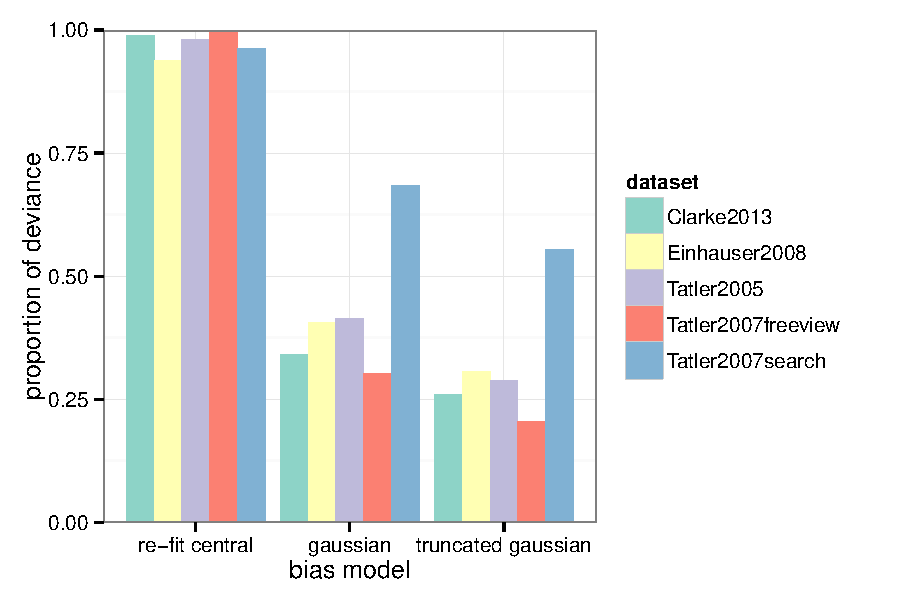
\includegraphics[width=12cm]{../scripts/flow/figs/llh_ALL.pdf}
\caption{Flow:normal log likelihood results. We can see that re-fitting the central-bias to each specific dataset offers little improvement over using the Clarke-Tatler model, while the flow model offers a substantial improvement.}
\label{fig:nFlowDevAll}
\end{figure*}

As the flow:normal model is significantly more complex, requiring nine times as many parameters, it is important to test for robustness. We can test how well our model generalises on testing it on other datasets, for example, \cite{borji2015}. 


\begin{figure*}
\centering
 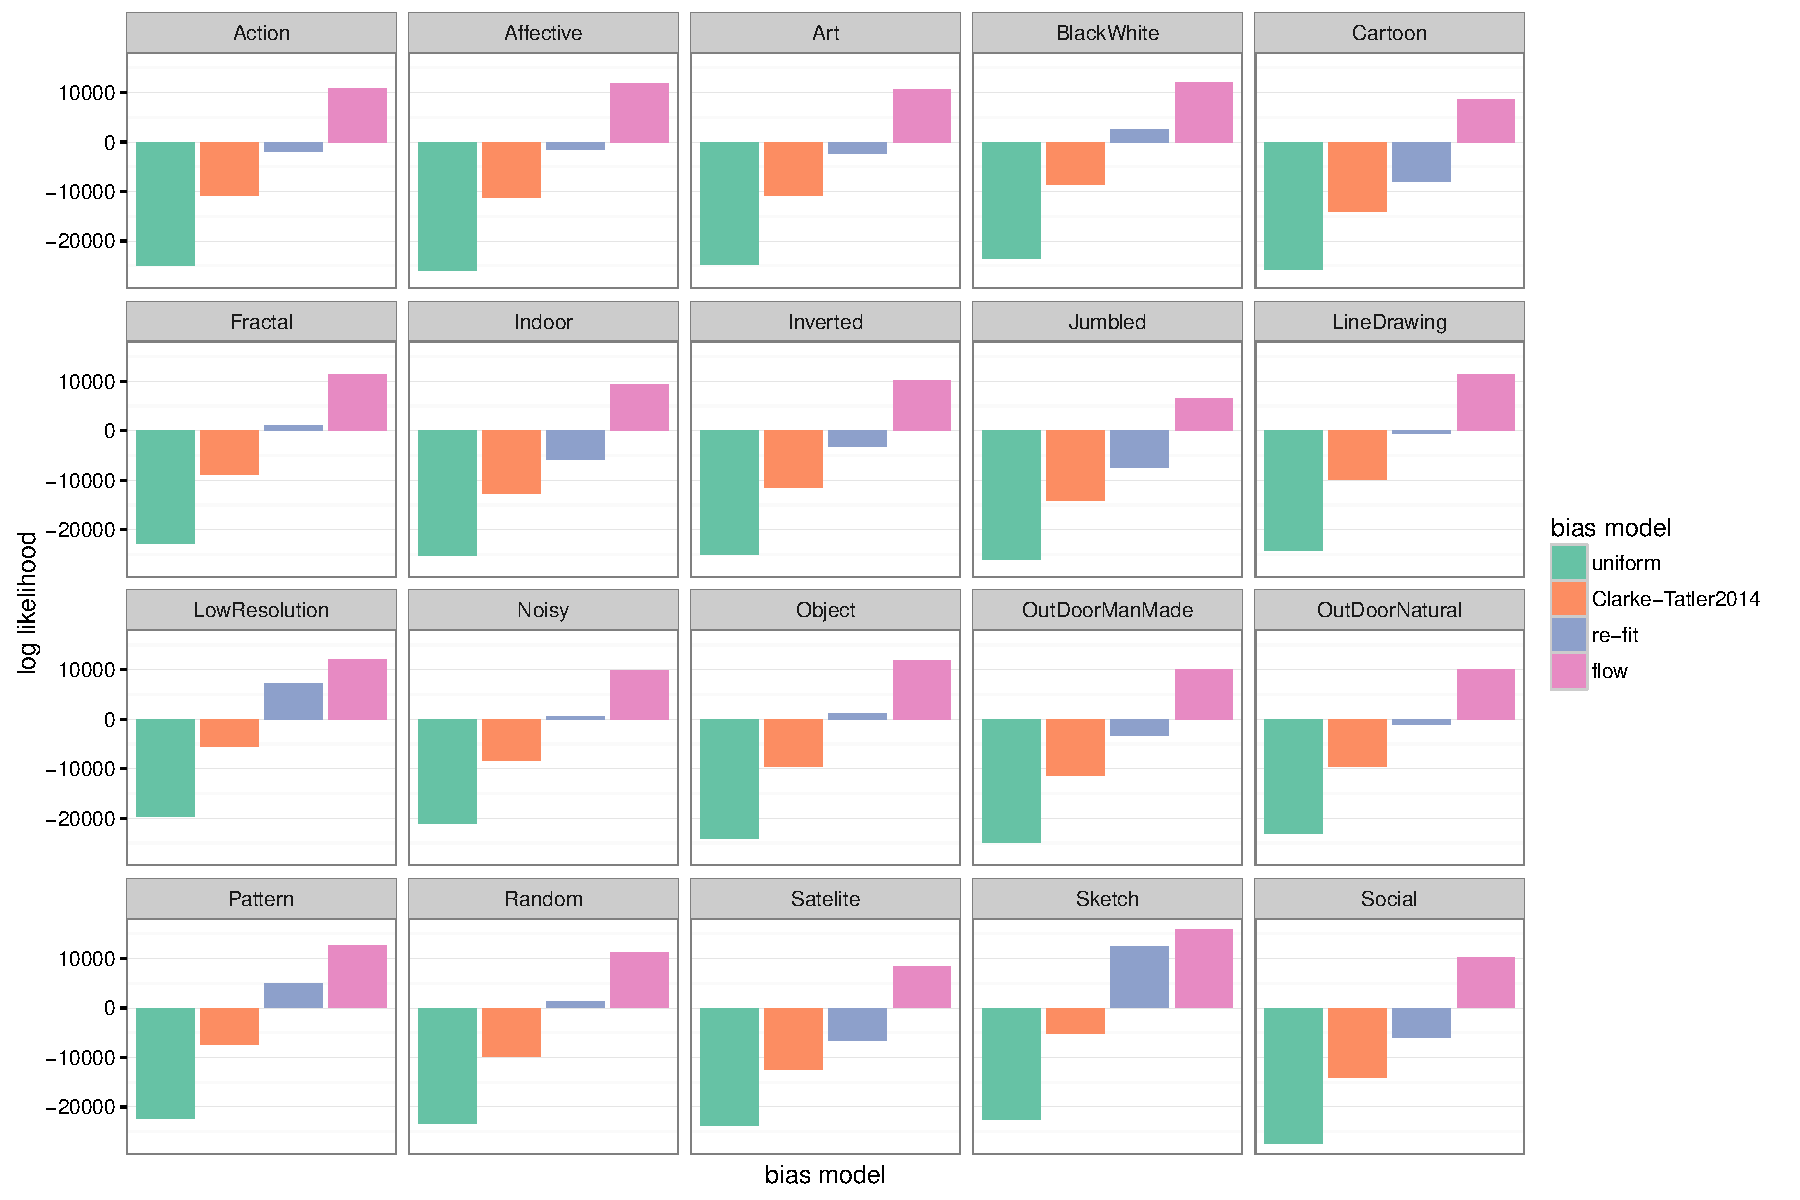
\includegraphics[width=12cm]{../scripts/flow/figs/llh_Borji.pdf}
\caption{Flow:normal deviance results. We can see that re-fitting the central-bias to each specific dataset offers little improvement over using the Clarke-Tatler model, while the flow:normal model decreases the deviance by half.}
\label{fig:nFlowDevBorji}
\end{figure*}

% \begin{figure}
% \centering
%  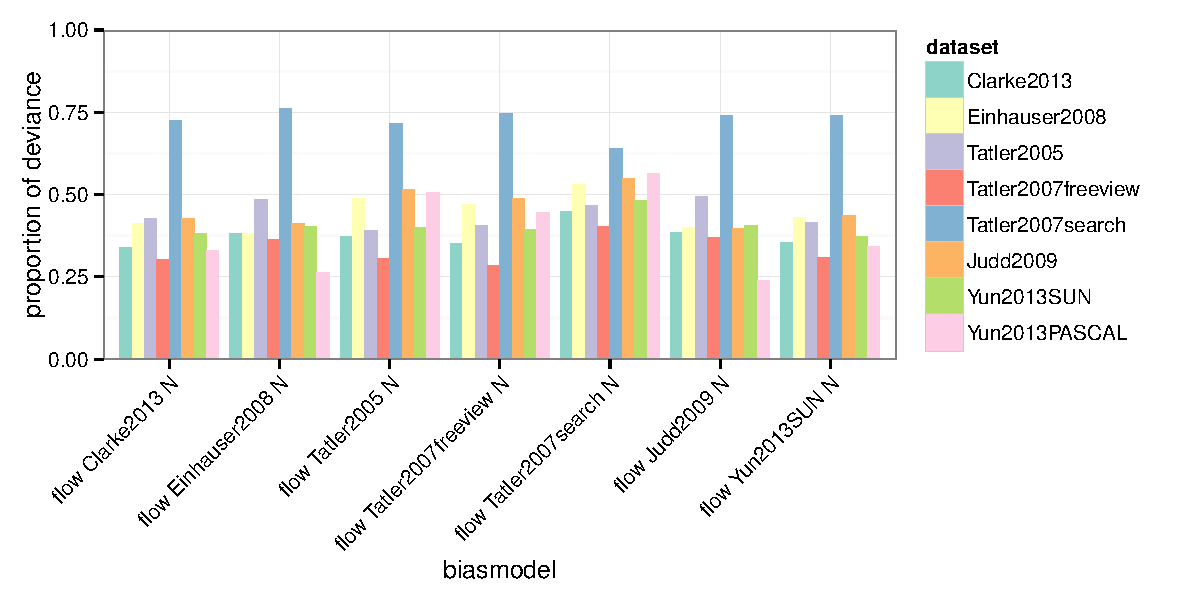
\includegraphics[width=12cm]{../scripts/flow/figs/llh_crossDataset.pdf}
% \caption{Flow:normal deviance results over datasets. In general, we can see that bias models trained on different datasets all explain around the same amount of variance in the datasets.}
% \label{fig:nFlowDevCross}
% \end{figure}

\subsubsection{Discussion}

We put the Flow:normal model forward as a robust prior for image-content independent saccadic behaviour. This model can be thought of as as partner of the Clarke-Tater central bias, and we expect that in some cases, the simpler central bias will be more appropriate, while in others, the more complex flow model is a better choice. We have demonstrated that although this model requires more parameters, it generalises well from one dataset to another and is a far better baseline for modelling a scan-path than the central bias.

There are two main simplifications to our modelling work. First of all, we are using an unbounded distribution (ie, $(x,y)\in \mathbb{R}^2$) to model bounded data. While it is possible to deal with this issue, by either applying a transform $(-1,1)\rightarrow \mathbb{R}$ (such as $z=log(\frac{x'}{1-x'})$, where $x'=\frac{x+1}{2}$), or fitting a truncated multivariate Gaussian, we decided that given the good performance of the model as is, it was not worth adding the additional complexities to our model at this time. 

The second simplification is that we are treating the data as normal. From Figure \ref{fig:empiricalSaccadicFlow} we can see that the data is clearly skewed, particularly in the corners. We will attempt to address these issues in the following section.